This appendix chapter will briefly discuss how to install, test, and run RegCM.
This chapter will also discuss how to access the User's Guide for RegCM.
Most of the instructions are already covered in the User's Guide,
	but the other parts that were not covered will be discussed here.

\section{Prerequisites}
	Since RegCM is a GNU-based system, a familiarity on how to use the Linux command line is a must.
	Also, since RegCM is written in Fortran, you need a Fortran compiler.
	
	The model needs at least two libraries:
	\begin{itemize}
		\item A netCDF Library 
		(\url{https://www.unidata.ucar.edu/software/netcdf/}),
		which you can test if it's installed by doing
		\texttt{nf-config --version},
		and
		\item MPI MPI Library
		(\url{http://www.openmpi.org/}),
		which you can test if it's installed by doing
		\texttt{ompi\_info --version ompi release}
	\end{itemize}
	The software is already installed on the desktops from Ubuntu
	repositories. You can find a script in the \texttt{Tools/Script} directory
	to compile required library from source.
	
	More on prerequisites are found in Section 3.1 and 3.2 of the User's Guide.
	
\section{Obtaining the Model and Documentation}
	According to the User's Guide, the packed archive file with the model code can be downloaded from the G-forge website: 
		\url{http://gforge.ictp.it/gf/project/regcm/frs}.
	However, I could not access the site myself.
	Instead, I had to go into the model's GitHub site:
	\begin{center}
		\url{https://github.com/ICTP/RegCM}
	\end{center}
	to download it.
	From the GitHub website, under ``Releases'', there will be a release entitled ``NH V5 code''.
	Click on that, and you will see a link to download either a \texttt{zip} package or a \texttt{tar.gz} package.
	Download the \texttt{tar.gz} package, and extract the files from those packages using
	\begin{center}
		\texttt{tar -zxvf RegCM-5.0.0.tar.gz}.
	\end{center}
	Alternatively, if your machine has \texttt{git} and you want the most updated version of RegCM, you can use \texttt{git pull} to download the source code directly from the most recent commit to the GitHub master branch.
	Do note though, that the source code from the Releases tab may be different from the most recent commits to the master branch.

\section{Accessing the User's Guide}
	Before doing this section, do a quick Google search or check the lab's files (NAS or Google Drive) to see if an updated version of the RegCM User's Guide is available online.
	If there is, then you don't need to compile the User's Guide yourself.

	The User's Guide does not come as a \texttt{pdf}.
	Instead, the User's Guide comes with the RegCM source code as \LaTeX\ code.
	You will need a \LaTeX\ distribution and compile the code yourself.
	I will not discuss how to install \LaTeX\ here, but this guide in StackExchange may be helpful to you:
	\begin{center}
		\url{https://stackoverflow.com/a/1017170}.
	\end{center}

	In the source code for RegCM, there is a folder called \texttt{Doc}.
	In that folder is the \LaTeX\ source code for the User's Guide, Developer Guide, and Reference Manual, and a commented version of the input file for RegCM.
	Use your \LaTeX\ distribution to compile the \texttt{UserGuide.tex} file under the \texttt{UserGuide} folder into a readable \texttt{pdf}.
	Following the User's Guide will be very helpful for setting up, testing, and running RegCM.
	
\section{Installing and Testing RegCM}
	from the RegCM root folder, you'll want to run the provided \texttt{configure} script by typing
	\begin{center}
		\texttt{./configure}
	\end{center}
	If you plan on using the Community Land Model 4.5 instead of the default Biosphere-Atmosphere Transfer Scheme, then you'll need to do 
	\begin{center}
		\texttt{./configure --enable-clm45}
	\end{center}
	instead.
	Then, you'll want to run
	\begin{center}
		\texttt{make install}
	\end{center}
	to install the software.
	For more detailed instructions, see Chapter 3 of the User's Guide.

\section{Downloading Global Datasets}
	Besides the time it takes to run RegCM itself, this step will take the most of your time.
	You will need various global datasets for RegCM's inputs.
	They can be found in
	\begin{center}
		\url{http://clima-dods.ictp.it/regcm4/}
	\end{center}
	and can be downloaded in the command line using either \texttt{curl} or \texttt{wget}.
	For example, to recursively download all files in a particular folder, you can use the \texttt{-r} and \texttt{-np} options for \texttt{wget} (which correspond to ``recursive'' and ``no parent'', respectively). 
	Also, it's VERY important to test if the files have downloaded properly, since sometimes the files may have been incompletely downloaded or have been corrupted.
	To do this, you can check with the \texttt{-c} option (which corresponds to ``continue'').
	Lastly, web crawlers are disallowed on the website for some bizzare reason!? So you'll need the \texttt{-e robots=off} option. 
	All in all, your download command might look like:
	\begin{center}
		\texttt{wget -c -r -np -e robots=off <url>}
	\end{center}
	Instead of recursion, you may also create a for loop to loop through multiple files.
	
	The datasets are BIG in size, and you may need to fill up about $\qty{100}{GB}$ of storage, maybe even more.
	Which datasets to download is up to your needs.
	For the datasets needed to test the model, please see Chapter 4 of the User's Guide.
	
\section{Running a Test Simulation}
	Running a test simulation using the model is covered in detail in Chapter 5 of the User's Guide, and will not be covered here.
	
	If you are using the CLM4.5 version of RegCM, then instead of the 
	\texttt{terrain}, \texttt{sst}, \texttt{icbc}, and \texttt{regcmMPI} programs,
	they will be replaced with 
	\texttt{terrainCLM45}, \texttt{sstCLM45}, \texttt{icbcCLM45}, and \texttt{regcmMPICLM45} programs.
	Furthermore, you will also need to run the \texttt{mksurfCLM45} program after running the \texttt{terrainCLM45} program.
	A summary of the inputs and outputs of RegCM are seen in the included schematic.
	\begin{figure}	
		\centering
		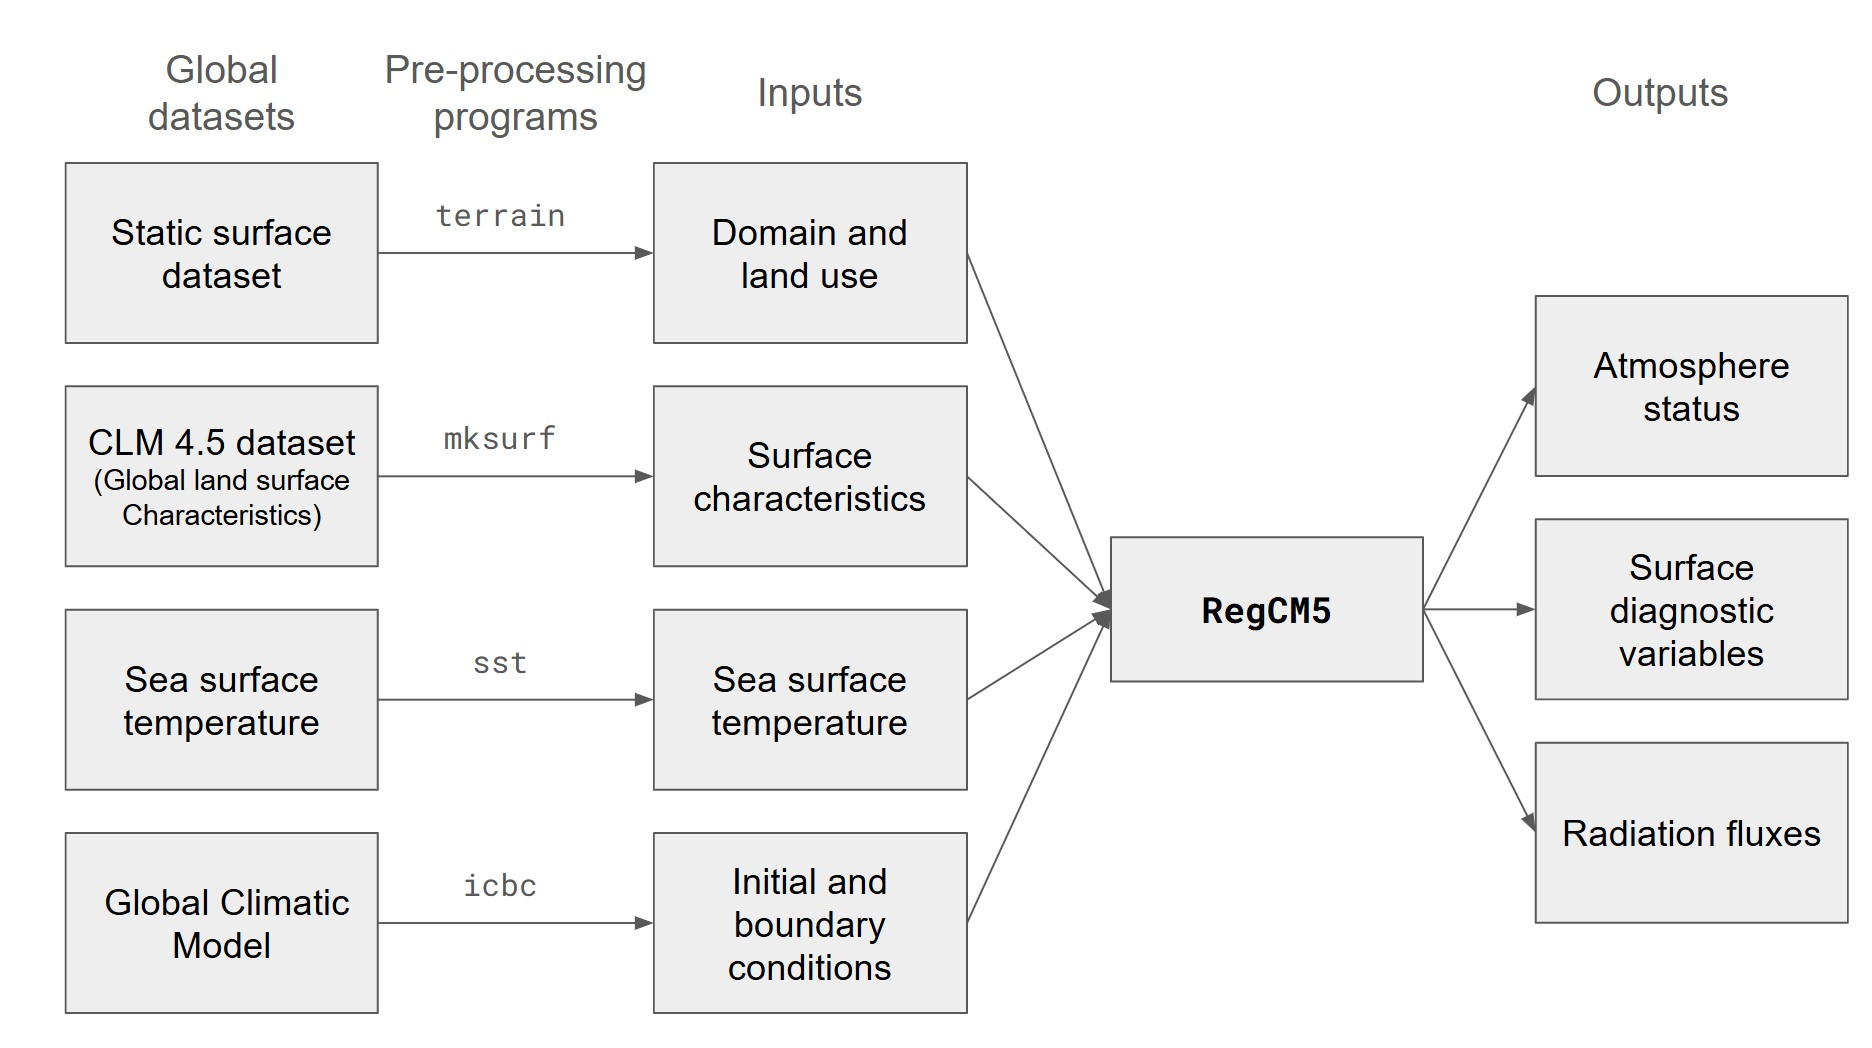
\includegraphics[width = \textwidth]{schematic-regcm-inputs-outputs}
		\caption{
			Schematic of the inputs and outputs of RegCM5 (with CLM 4.5)
		}
	\end{figure}
	
\section{Changing Settings and Running Your Own Simulations}
	RegCM parameters are covered in Chapter 6 of the User's Guide, and will not be covered here.
	Running your own simulation will be similar to running the test simulation, but now you have free reign to change parameters to fit your experiments.
	
	RegCM can be very computationally intensive, especially if you use a high number of CPU cores (and your machine might crash! It has happened to me multiple times).
	So you can run chunks of the simulation at a time using the 
	\texttt{\&restartparam} section, where \texttt{ifrest = .false.} indicates a first run, and \texttt{ifrest = .true.} indicates subsequent runs.
	When continuing a run:
		First set \texttt{ifrest} to \texttt{.true.},
		set \texttt{mdate1} to the value in \texttt{mdate2},
		and then
		define the new value for \texttt{mdate2}.
	I recommend doing small time intervals at a time (try one month first), then doing larger time intervals (two months, then three, \dots) to see how well your machine can handle RegCM.
	
	A good chosen \texttt{dt} is important, as a value too big will make the simulation stop, but a value too small will make the simulation take forever.
	As a rule of thumb, try a \texttt{dt} value not greater than three times the \text{ds} value.
	If the simulation tells you to use a lower value, then decrease it and rerun the simulation.
	
\section{Final Tips}
	Most of your time will be spent on waiting\dots\ and waiting\dots\ and waiting\dots.
	So be sure to plan your downloads/runs accordingly.
	Make sure that the datasets are properly downloaded and not incomplete/corrupted.
	Make sure to regularly check on your simulations to see if they are still running.
	Have an external drive handy so you can transfer the big output file from the machine when it's done.
	You can have multiple machines downloading datasets and then just transfer them to other machines as needed.
	Good luck!